\documentclass[11 pt , a 4 paper ]{article}
\usepackage[dvipsnames]{xcolor}
\usepackage{tikz}
\usetikzlibrary{shapes}
\usetikzlibrary{calc}
\usepackage{anyfontsize}
\usepackage{sectsty}
\usepackage{graphicx} % Required for inserting images
\usepackage{amsmath} % AMS Base Package
\usepackage{amssymb} % AMS Symbols
\usepackage{amsthm} % AMS
\usepackage{hyperref} % Hyperrefferings
\usepackage{amsfonts} % AMS Fonts
\usepackage{tabto}
\usepackage{enumitem}
\usepackage[utf8]{inputenc}
\usepackage{pgfplots} % Plots
\pgfplotsset{width=10cm,compat=1.9}
\usepackage[margin=1cm]{geometry}
\usepackage[skins]{tcolorbox}
\usepackage{listings}  %Code blocks
\usepackage{enumitem} % Fancy Bullet points
\usepackage{array} %Tables
\usepackage{xcolor} % Text Color
\usepackage{svg}
\usepackage{pdfpages}
\usepackage{array} %Tables
\usepackage[table]{xcolor} % Text Color
\usepackage{float}
\usepackage{booktabs} % For professional horizontal lines
\usepackage{siunitx}  % For aligning numbers on the decimal point
\usepackage[table]{xcolor} % For adding color (e.g., zebra stripes)
\usepackage{tabularx} % For tables that adjust to a specific width
\usepackage{ragged2e} % for '\RaggedRight' macro (suppress full justification)
\usepackage{booktabs} % for '\toprule', '\midrule', and '\bottomrule' macros

\definecolor{aqua}{RGB}{3,164,186}
\definecolor{grey}{RGB}{200,200,200}


{\Huge\title {CSIT123 - Computing and Cyber Security Fundamentals}}

\author{Ruhan Shafi}
\date{\today}

\theoremstyle{definition}
\newtheorem{thm}{Defination}


\usepackage{xcolor}

\definecolor{codegreen}{rgb}{0,0.6,0}
\definecolor{codegray}{rgb}{0.5,0.5,0.5}
\definecolor{codepurple}{rgb}{0.58,0,0.82}
\definecolor{backcolour}{rgb}{0.95,0.95,0.92}

\lstdefinestyle{mystyle}{
	backgroundcolor=\color{backcolour},   
	commentstyle=\color{codegreen},
	keywordstyle=\color{magenta},
	numberstyle=\tiny\color{codegray},
	stringstyle=\color{codepurple},
	basicstyle=\ttfamily\footnotesize,
	breakatwhitespace=false,         
	breaklines=true,                 
	captionpos=b,                    
	keepspaces=true,                 
	numbers=left,                    
	numbersep=5pt,                  
	showspaces=false,                
	showstringspaces=false,
	showtabs=false,                  
	tabsize=2
}

\lstset{style=mystyle}
\begin{document}
		\pagestyle{empty}
		\begin{tikzpicture}[remember picture,overlay]
				\fill[BlueViolet] (current page.south west) rectangle (current page.north east);
				\begin{scope}
						\foreach \i in {2.5,...,22}
						{\node[rounded corners,BlueViolet!90,draw,regular polygon,regular polygon sides=6, minimum size=\i cm,ultra thick] at ($(current page.west)+(2.5,-5)$) {} ;}
					\end{scope}
				\node[rounded corners,fill=BlueViolet!95,text =BlueViolet!5,regular polygon,regular polygon sides=6, minimum size=2.5 cm,inner sep=0,ultra thick] at ($(current page.west)+(2.5,-5)$) {{\includegraphics[scale=.06]{~/Notes/LaTex Work/logo4.png}}};
				\foreach \i in {0.5,...,22}		
				{\node[rounded corners,BlueViolet!90,draw,regular polygon,regular polygon sides=6, minimum size=\i cm,ultra thick] at ($(current page.north west)+(2.5,0)$) {} ;}
				\foreach \i in {0.5,...,22}
				{\node[rounded corners,BlueViolet!98,draw,regular polygon,regular polygon sides=6, minimum size=\i cm,ultra thick] at ($(current page.north east)+(0,-9.5)$) {} ;}
				\foreach \i in {12}
				{\node[fill = BlueViolet
						,rounded corners,draw=BlueViolet,regular polygon,regular polygon sides=6, minimum size=\i cm,ultra thick] at ($(current page.south east)+(-0.2,-0.45)$) {} ;}
				\foreach \i in {21,...,6}
				{\node[BlueViolet!95,rounded corners,draw,regular polygon,regular polygon sides=6, minimum size=\i cm,ultra thick] at ($(current page.south east)+(-0.2,-0.45)$) {} ;}
				\node[left,BlueViolet!5,minimum width=0.625*\paperwidth,minimum height=3cm, rounded corners] at ($(current page.north east)+(0,-9.5)$){{\fontsize{25}{30} \selectfont \bfseries Assessment 2 Lab Report}};
				\node[left,BlueViolet!10,minimum width=0.625*\paperwidth,minimum height=2cm, rounded corners] at ($(current page.north east)+(0,-11)$){{\huge \textit{Foundations of Robotics}}};
				\node[left,BlueViolet!5,minimum width=0.625*\paperwidth,minimum height=2cm, rounded corners] at ($(current page.north east)+(0,-13)$){{\Large \textsc{Ruhan Shafi}}};
			\end{tikzpicture}
	\newpage
	\ \vskip -1cm
	\rightline{\includegraphics[scale=.06]{~/Notes/LaTex Work/logo3.png}}
	
	\vskip -40pt
	
	\noindent
	{Foundations of Robotics | Ruhan Shafi (u3284342)}
	
	\vskip 5pt
	
	\noindent{\bf\Large Assessment 2: Lab Report}
	
	\vskip 7pt
	{\color{aqua}\hrule height 1pt}
	{\color{grey}\hrule height 1pt}
	
	\vskip 5pt

  \section*{Task 1 - Localisation, Navigation \& Path Planning using Mobile Robots}

  \subsection*{Localisation Example}
  \textbf{1D Bayesian Localisation with Noisy Sensors and Motion}\\
  \newline \noindent This cell sets up and begins to demonstrate the core concept of Bayesian localisation in a simplified one-dimensional world. The world is represented as a line of 100 positions, and the robot is given 20 simulated measurement readings spaced evenly across that world (via \texttt{np.linspace}), with a small amount of integer noise added to simulate a real, imperfect sensor. Alongside the measurements, a motion array is created representing how far the robot moves between each step, again with noise to simulate imperfect odometry. The key parameters \texttt{pHit} (0.6) and \texttt{pMiss} (0.2) define the sensor model - the probability that the sensor correctly identifies the robot's true location versus reporting a wrong one. Similarly, \texttt{pExact}, \texttt{pUndershoot}, and\texttt{pOvershoot} define how reliable the robot's movement is. \\ 
  \newline \noindent The belief is initialised as a uniform distribution (\texttt{np.ones(world\_size) / world\_size}) meaning the robot has no idea where it is and considers every position equally likely. This flat line plotted in the initial figure is the robot's prior: maximum uncertainty. The loop that follows performs the Bayesian update cycle. For each time step, a likelihood array is computed by assigning \texttt{pHit} to the cell matching the current measurement and \texttt{pMiss} to every other position. This likelihood is then multiplied into the belief (element-wise), and the result is renormalised so all probabilities still sum to one. This is the measurement update step of the Bayes filter, the robot's belief sharpens around positions that are consistent with what the sensor reported. This cell directly demonstrates how probability theory allows a robot to reason about where it is even when both its sensors and motors are noisy, which is the foundational challenge of localisation.

  \begin{center}
    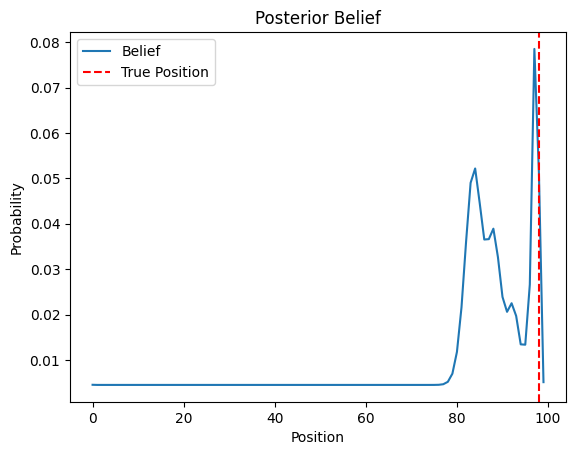
\includegraphics[scale=0.5]{1.png}
  \end{center}
  \textbf{Building a 2D World and Placing Particles}\\
  \newline \noindent Cell 8 constructs the 2D environment used for the particle filter demonstration. A \texttt{50×50} grid is initialised to zero (free space), and then four landmark positions are randomly generated and placed into the grid by setting their cells to $1$. These landmarks are then "grown" by three iterations of \texttt{np.roll}, a trick that shifts the landmark array by one cell in each direction and OR-combines the result with the original, effectively expanding each landmark into a small blob. This makes the landmarks physically larger and more realistic to detect. A robot is then placed at a random position and displayed as a red dot on the map. This environment establishes the ground truth that the particle filter will try to reason about. \\
  \newline \noindent Cell 10 creates the particle filter's initial belief state. Thirty particles are randomly scattered across the free cells of the map, with any particles that land on a landmark immediately resampled to a free position, ensuring all hypothesised robot positions are physically valid. Each particle is assigned an equal weight of \texttt{1/num\_samples}, reflecting total uncertainty about where the robot actually is. When displayed, all particles appear with the same shade (equal weight), scattered uniformly across the environment. Together, cells 8 and 10 establish the two-layer nature of particle filters: the real world (the map with landmarks and the robot's true position) and the belief representation (the cloud of weighted hypotheses). The robot knows the map but does not know which particle represents its true location, that is what the filter must figure out.
  \begin{center}
    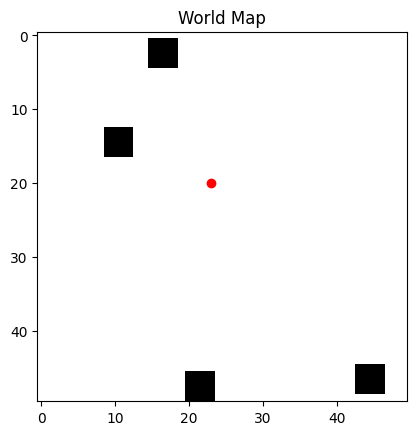
\includegraphics[scale=0.5]{1a.png}
    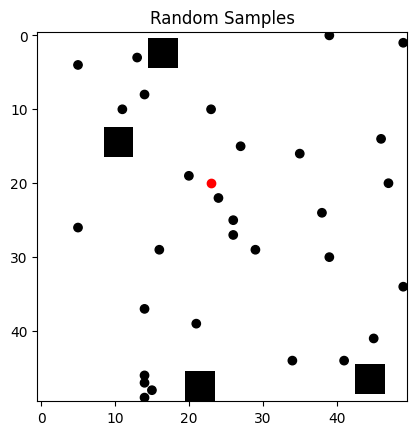
\includegraphics[scale=0.5]{1b.png}
  \end{center}
  \textbf{Particle Weight Update via Gaussian Likelihood}\\ 
  \newline \noindent This cell is the heart of the particle filter — the measurement update step. The robot first takes a "measurement" of the real world by computing its actual Euclidean distance to each of the four landmarks using \texttt{np.linalg.norm}. This represents what the robot's range sensor actually reads. For each particle (each hypothesised robot position), the function \texttt{sample\_probability} computes how likely that particle's position could have produced the robot's observed measurements. It does this by calculating what the distance to each landmark would be if the robot were at that particle's location, then evaluating a Gaussian probability density function comparing that expected distance to the actually observed distance. A particle that is close to the robot's true position will predict distances similar to the observed distances, yielding a high probability; a particle far from the true position will predict very different distances, yielding a low probability.\\ 
  \newline \noindent The resulting probabilities for each landmark are summed to produce a single weight per particle, and all weights are then normalised to sum to one. The weighted centroid of the particles, computed with \texttt{np.average} using weights, gives the current best estimate of the robot's position. This process directly implements the Bayesian update: \texttt{posterior $\alpha$ likelihood $\times$ prior}. The prior is the particle distribution from the previous step; the likelihood is the Gaussian sensor model; and the posterior is the new set of weights that concentrate probability mass around particles consistent with the observation. In a real AMCL system running in ROS, this same principle operates at every sensor update step, with particles that better explain the laser scan receiving higher weights and being more likely to survive the subsequent resampling step.
  \begin{center}
    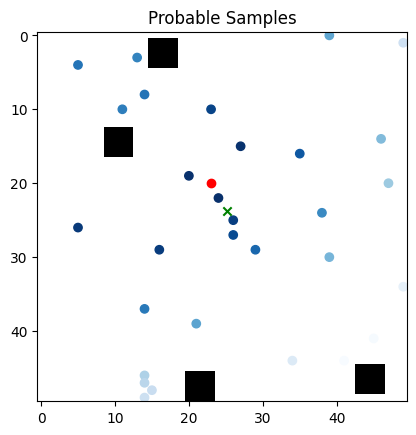
\includegraphics[scale=0.5]{1c.png}
    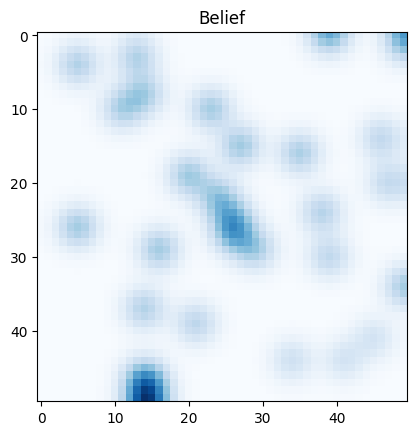
\includegraphics[scale=0.5]{1d.png}
  \end{center}
  \subsection*{Mapping Example}
  \subsubsection*{Code Breakdown \& Application}
   \noindent This cell implements a complete occupancy grid mapping pipeline across four functions that work together to simulate how a robot builds a map of an unknown environment using a laser scanner and known movement. The \texttt{generate\_obstacle\_map} function constructs the ground truth world, a 20×20 grid with perimeter walls and three internal obstacles, which the robot has no direct access to and must discover entirely through sensing. The \texttt{simulate\_laser\_scan} function models a 360$\deg$ lidar by casting 36 rays outward from the robot's position using trigonometry, stepping along each ray until it hits an obstacle or exceeds the maximum range of 10 cells, recording the distance to each hit and storing NaN for rays that return nothing. The \texttt{update\_occupancy\_grid} function then takes those hit distances, converts them from polar back to absolute Cartesian grid coordinates, and increments the corresponding cell in the occupancy grid by one, each hit is effectively a vote that a cell is occupied, with cells observed multiple times accumulating higher counts and appearing darker. Finally, \texttt{simulate\_mapping\_with\_iterations} ties everything together by moving the robot through six hard-coded positions, calling scan and update at each stop, and rendering the progressive state of the map across six subplots before producing a final side-by-side comparison with the ground truth. Because all robot positions are supplied directly, this is pure odometry-based mapping, the robot is assumed to know exactly where it moved, completely removing localisation uncertainty from the problem. \\ 
  \newline \noindent When this cell runs, the six subplots make the incremental nature of mapping immediately tangible: early iterations show only sparse clusters of detected cells near the starting position, and the map fills progressively as the robot traverses the space but even at the end it never perfectly matches the ground truth, because the single-point obstacle at (15, 15) may fall between ray directions and go undetected, far corners remain white because the robot never moved close enough to scan them, and the coarse 10$\deg$ angular resolution leaves geometric blind spots throughout. This is precisely what real-world mapping looks like on physical hardware, and the pipeline here is a direct conceptual replica of what runs on an actual robot. The \texttt{simulate\_laser\_scan} function is replaced by a physical lidar, such as an RPLIDAR or Velodyne, publishing \texttt{sensor\_msgs/LaserScan} messages on the \texttt{/scan} ROS 2 topic at 10-15 Hz, and the occupancy grid update logic mirrors what SLAM systems like Cartographer compute probabilistically on every scan callback, publishing the result as a \texttt{nav\_msgs/OccupancyGrid} on the \texttt{/map} topic for RViz to visualise and Nav2 to consume for path planning. The critical limitation exposed by the final comparison, that perfect odometry does not exist on real robots, is exactly why SLAM replaces this approach in deployment: rather than assuming known positions, systems like Cartographer simultaneously correct the robot's pose estimate by matching new scans against the already-built map, closing loops when the robot revisits a known area and globally re-optimising the entire trajectory to prevent accumulated drift from warping the map into something unusable for navigation.
  \begin{center}
    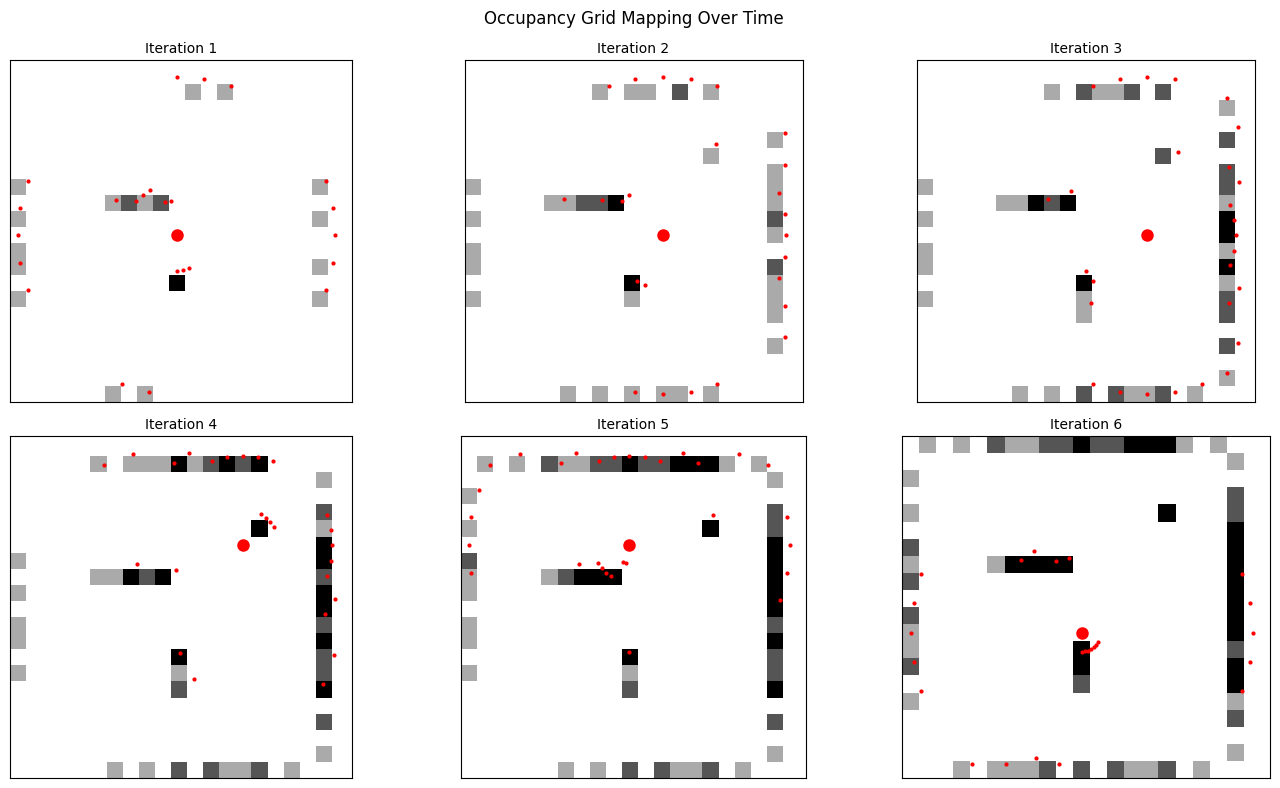
\includegraphics[width=\textwidth]{2a.png}
    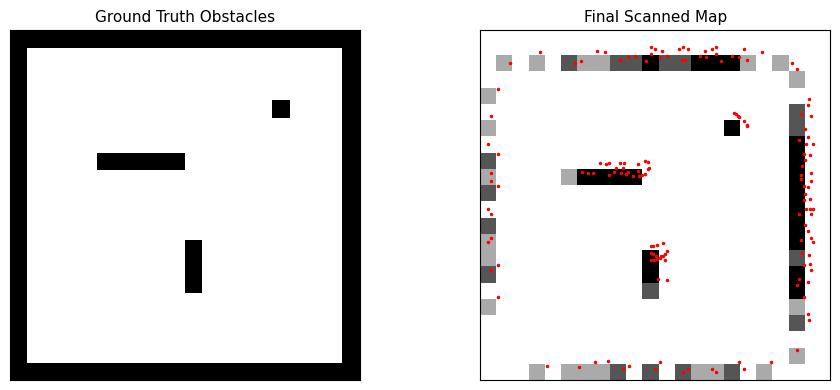
\includegraphics[width=\textwidth]{2b.png}
  \end{center}

  \textbf{Review Questions}
  \begin{enumerate}
    \item What is the main advantage of using an occupancy grid over a feature-based (graph) representation?\\
    \newline \noindent The main advantage of an occupancy grid is its ability to represent arbitrary, unstructured environments in a dense and complete way, without requiring the environment to contain any identifiable landmarks or geometric features. Every cell in the grid independently stores an estimate of whether that region of space is occupied, free, or unknown, making it straightforward to represent cluttered, irregular spaces. A feature-based or graph representation, by contrast, only stores discrete landmarks or nodes and the edges between them, which means the map is only as good as the distinctiveness of features the robot can detect.\\ 
\newline \noindent Consider a completely open, featureless hallway as an example. In an occupancy grid, this hallway would be represented as a long rectangular region of free (white) cells, flanked on either side by occupied (black) cells corresponding to the walls, with unknown (grey) cells beyond the sensor's range. The representation is natural and complete even though the hallway has no distinctive geometry. In a feature-based representation, however, a featureless hallway is deeply problematic. There are no corners, objects, or distinctive points to serve as landmarks, so the graph would contain little or no nodes within the hallway itself. The robot would struggle to localise within this stretch because it cannot match current observations to any stored features, leading to what is known as the "perceptual aliasing" or "featureless environment" problem.
    \item In the example above, the robot has perfect odometry (knows exactly where it moved). What happens in real robots that don't have perfect odometry?\\
     \newline \noindent In real robots, odometry errors accumulate continuously as the robot moves. Each small error in measuring wheel rotation or angular velocity compounds with every subsequent step through a process called dead reckoning drift. Over short distances this is often manageable, but over longer trajectories the estimated pose can deviate substantially from the true pose. The practical consequence for mapping is that sensor readings such as lidar scans, depth images, or sonar returns, are placed into the map according to the robot's estimated pose. If that estimate is wrong, the readings are placed in the wrong location. Walls appear curved or doubled, corridors seem to bend when they are straight, and when the robot completes a loop and returns to a previously mapped area, the two versions of the same wall may not align, creating a "ghost" duplicate in the map. This is the classic loop closure problem: without correcting for accumulated drift when a known place is revisited, the map becomes globally inconsistent even if it looks locally reasonable.
    \item Why are some obstacles not detected even though the robot passed nearby them?\\
      \newline \noindent Some obstacles remain undetected because they fall outside the effective range of the laser scanner. A lidar sensor has a maximum range beyond which it cannot reliably return valid measurements. Any obstacle that is further from the robot than this range limit at the time of every scan will never be hit by a laser beam, and therefore will never be marked as occupied. Additionally, lidar operates on a line-of-sight principle: if an obstacle is occluded behind another object from every vantage point the robot occupied, it will never be directly observed. Areas that the robot never drove close enough to, such as far corners of rooms, spaces behind large furniture, or regions at the ends of long corridors that were only traversed at one end, will remain as unexplored grey or white space in the map even though the robot technically passed in their general vicinity.
    \item The occupancy grid is updated by incrementing cells where obstacles are detected. How would you modify this to include uncertainty?\\
      \newline \noindent An example of a simple counting approach that addresses this problem is the following. Increment a cell each time an obstacle is detected there and decrement it when a ray passes through it freely, is intuitive but does not properly capture uncertainty or allow for principled fusion of conflicting evidence. A more rigorous approach is to use a probabilistic framework based on log-odds updates. In this scheme, each cell stores the log-odds of it being occupied, which is the logarithm of the ratio of the probability of occupancy to the probability of being free. When a sensor ray terminates at a cell (indicating an obstacle), a positive log-odds value is added; when a ray passes through a cell without hitting anything (indicating free space), a negative log-odds value is added. This is computationally efficient because updates are additions rather than multiplications, and it naturally saturates, a cell that has been observed as free many times will have a very low log-odds value, making it resistant to being flipped by a single spurious reading, while a cell consistently observed as occupied will be highly confident. This approach also handles sensor noise gracefully, because a single uncertain observation only slightly shifts the probability, and a consistent pattern of observations is required to reach a high-confidence determination.
    \item In real-world robotics, mapping is coupled with localization (SLAM - Simultaneous Localization and Mapping). Why can't we just use pure odometry for long-term mapping missions\& What problems arise from odometry drift?\\ 
      \newline \noindent Pure odometry is fundamentally unsuitable for long-term mapping missions because its errors are unbounded and they grow without limit as a function of distance travelled and time elapsed. Wheel encoders are affected by wheel slip on uneven terrain, different floor materials, or when turning, all of which cause the measured arc length to differ from the actual distance moved. IMUs suffer from gyroscope bias and accelerometer noise, and integrating these noisy signals to obtain velocity and then position causes errors to grow as the square root of time (for random noise) or even linearly (for systematic bias). Over the course of a long mission, what starts as a centimetre-level position error becomes a metre-level error and then larger still. For a mapping mission, this means the map progressively warps and distorts, with later observations being placed increasingly far from their true positions. In a warehouse, hospital, or large outdoor environment where the robot might traverse hundreds of metres or operate for hours, a pure odometry map would be entirely unusable for navigation by the end of the mission.
  \end{enumerate}
  \subsection*{SLAM Example}
   \begin{center}
    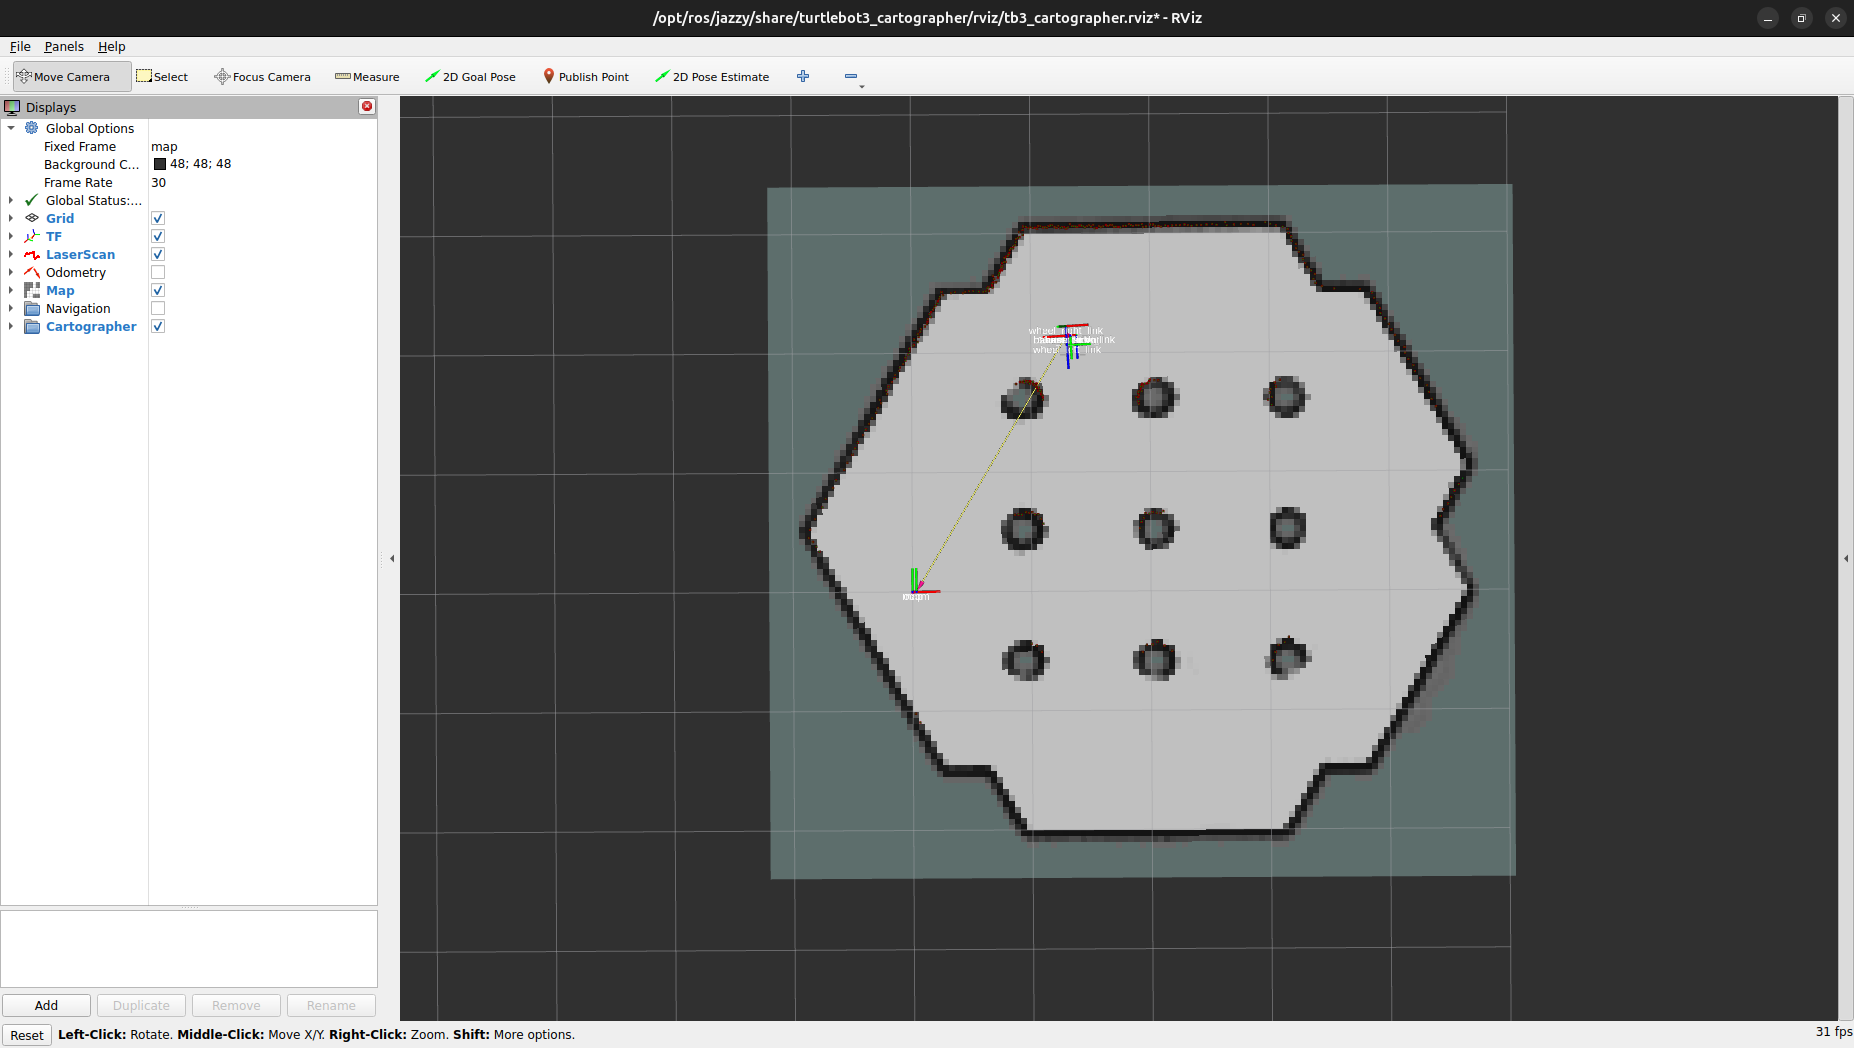
\includegraphics[scale=0.25]{Pasted image.png}
  \end{center}
  \textbf{Review Questions}
  \begin{enumerate}
    \item What is the difference between mapping and SLAM?\\ 
      \newline \noindent Mapping and SLAM are related but distinct problems in robotics. Mapping refers to the process of building a representation of the environment, but it assumes that the robot's position is already known at every point in time. In other words, pure mapping takes a known trajectory as input and produces a map as output. SLAM, which stands for Simultaneous Localisation and Mapping, tackles both problems at once: the robot must build a map of an unknown environment while simultaneously figuring out where it is within that map. The two problems are deeply intertwined, you need a map to localise, and you need to know your location to build an accurate map, which is precisely what makes SLAM a fundamentally harder problem than mapping alone.
    \item Why is SLAM considered more challenging than mapping alone?\\
    \newline \noindent SLAM is more challenging because the robot lacks two critical pieces of information at the same time: it does not know the map, and it does not know its own precise location within that map. In pure mapping, the robot is given ground-truth pose information (perhaps from GPS, motion capture, or a pre-surveyed trajectory), so it only needs to interpret sensor readings and place them correctly in the world frame. In SLAM, the robot only has access to its odometry (wheel encoders, IMU readings, etc.) and its onboard sensors such as lidar or cameras. Odometry is inherently noisy and accumulates drift over time, meaning the robot's estimated position diverges from its true position. Because the map is built on top of these noisy pose estimates, errors in localisation propagate directly into the map, and errors in the map in turn degrade localisation. The robot must jointly estimate both the map and its own trajectory, resolving this circular dependency in real time, often under strict computational constraints.
    \item What sensor(s) does cartographer use as input to build maps?\\ 
      \newline \noindent Google Cartographer is primarily designed around 2D and 3D lidar as its core input sensor. It processes laser scan data to detect the geometry of the surrounding environment and builds a submap-based representation of the world. In addition to lidar, Cartographer can also incorporate data from an Inertial Measurement Unit (IMU), which provides high-frequency measurements of acceleration and angular velocity. The IMU data helps constrain the robot's pose estimate between lidar scans, particularly for handling rotational motion and dealing with the motion distortion that occurs in spinning lidars while the robot is moving. Odometry data from wheel encoders can also be fused in as an optional additional input. The combination of lidar and IMU makes Cartographer robust to fast robot motions and gives it the ability to perform both 2D occupancy grid mapping and full 3D mapping depending on the sensor configuration.
    \item How would SLAM perform if the robot had perfect odometry (zero drift)?\\ 
      \newline \noindent If a robot had truly perfect odometry, meaning it knew its exact position and orientation at every instant with zero error and zero drift,  the localisation half of the SLAM problem would effectively be solved. The robot would always know precisely where it was in the world frame, so it could directly project every sensor reading onto the correct location in the map without needing to perform any pose correction or loop closure. In this idealised scenario, pure mapping would suffice and SLAM in its full sense would not be strictly necessary. However, perfect odometry is physically impossible in real systems. Wheel slip, surface irregularities, encoder quantisation, IMU bias, and integration errors all cause odometry to drift unboundedly over time. Even small per-step errors accumulate into large global errors over long distances. SLAM is therefore necessary precisely because real odometry is imperfect, and the robot must use environmental observations, such as recognising a previously visited place — to correct its accumulated drift and maintain a globally consistent map.

  \end{enumerate}
  \subsection*{Part B - A* algorithm visualizer}

  All the code used can be found on my Github including a video demonstration, linked \href{https://github.com/RuhanShafi/Dynamic-A-star}{here}.
  \begin{center}
    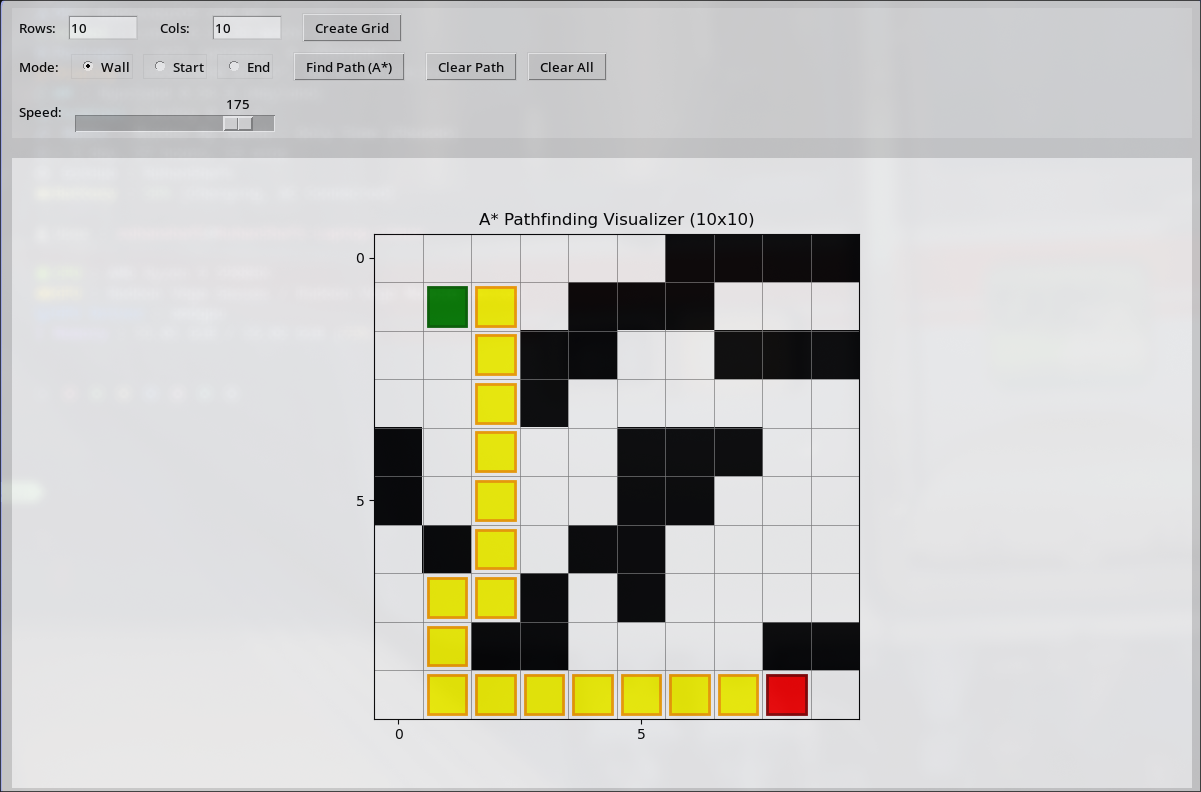
\includegraphics[scale=0.35]{Astar.png}

  \end{center}
 \noindent \textbf{Review Questions}
 \begin{enumerate}
   \item What do $g(n)$, $h(n)$, and $f(n)$ represent? Why is $f(n) = g(n) + h(n)$ important?\\
     \newline \noindent In the A* Algorithm, $g$ represents the accumulated real distance (or movement cost) along the path that has been traversed from the starting node to any given node $(n)$. The value $h(n)$ is the heuristic estimate of the cost from the current node to the goal, commonly computed as the Manhattan distance or Euclidean distance to the target cell. The value $f(n)$ is the total estimated cost of the cheapest path through the current node, combining what is known (the actual cost so far) with what is estimated (the remaining cost to goal). \\ 
     \newline \noindent The equation $f(n) = g(n) + h(n)$ is critical because it provides a principled way to prioritise which node to explore next. A* always expands the node with the lowest $f(n)$ value from its open list. By including $g(n)$, the algorithm remains aware of path cost and avoids unnecessarily long detours; by including $h(n)$, it is guided towards the goal rather than exploring blindly in all directions. The mathematical guarantee of A* — that it finds the shortest path — holds as long as $h(n)$ is admissible, meaning it never overestimates the true remaining cost. When $h(n) = 0$, A* degenerates into Dijkstra's algorithm (exhaustive cost-based search); when $g(n) = 0$, it degenerates into a greedy best-first search (fast but not guaranteed optimal).
   \item What do $0$ and $1$ mean in the maze? How does the algorithm avoid obstacles?\\ 
     \newline \noindent Within the  maze representation, $0$ denotes a free, traversable cell or "location" the robot is permitted to move through, while $1$ denotes an obstacle or wall, a cell that is blocked and impassable. When A* generates the neighbours of the current cell, it checks each candidate position: if the cell contains a $1$, it is immediately skipped and never added to the open list. This means that an obstacle cell can never be considered as a valid next step, which is how this algorithm avoids obstacles. Only cells containing $0$ that also fall within the grid boundaries are eligible for expansion, so the resulting path is inherently obstacle-free by construction.
   \item Why is diagonal movement allowed? What real-world scenarios does this represent?\\ 
     \newline \noindent The algorithm checks 8 adjacent positions, the four cardinal directions (up, down, left, right) and the four diagonal directions (top-left, top-right, bottom-left, bottom-right). Diagonal movement is allowed because it more accurately models the continuous 2D motion capabilities of real mobile robots. A ground robot, drone, or autonomous vehicle is not restricted to moving only parallel to a grid axis; it can move at any angle. By including diagonals, the algorithm can find shorter, more natural-looking paths that cut corners rather than taking unnecessarily angular routes. Real-world scenarios this represents include an autonomous warehouse robot navigating between shelving units at arbitrary angles, a drone flying through open airspace, a self-driving car changing lanes diagonally, or a robotic lawnmower cutting across an open area. In a 4-connected grid (no diagonals), paths often look unnaturally "staircase-shaped" even in open space, which would translate to inefficient and jerky robot motion.
   \item Why is A* more efficient than exploring every cell? How does $h$ guide the search?\\ 
     \newline \noindent Exploring every cell corresponds to a brute-force search (such as Breadth-First Search or exhaustive flood-fill), which in the worst case visits every reachable cell in the map before finding the goal. In a large occupancy grid this is computationally expensive and scales poorly. A* is more efficient because the heuristic $h$ provides directional bias, the algorithm preferentially expands nodes that appear to be closer to the goal, effectively concentrating the search effort in the geometrically relevant part of the map. Cells that are in the opposite direction from the goal accumulate high $f$ values and are therefore deprioritised or never explored at all. In practice, A* on a well-formed map typically explores only a fraction of the total cells, with the explored region forming a rough "cone" shape pointing from start toward goal. The efficiency gain is most dramatic in large open environments; in narrow mazes with few alternative paths, A* may still need to explore most of the map.
   \item What happens if no path exists? How could you detect and report this?\\ 
     \newline \noindent If the goal is completely enclosed by obstacles or is otherwise unreachable from the start, A* will exhaust its open list and it will run out of nodes to expand before ever reaching the goal. In a correctly implemented A*, this is detectable by checking whether the open list becomes empty before the goal node is popped. The current code can be modified to handle this by adding a check after the main loop: if the loop exits because the open list is empty (rather than because the goal was found), the algorithm should return a failure signal rather than an empty or partial path. In Python this might look like returning \texttt{None} or an empty list with a printed message such as \texttt{"No valid path found from start to goal"}. This is particularly important in robotics because sending a robot on a navigation task with no reachable goal could cause it to spin indefinitely or enter an error state; detecting the unreachable case allows the higher-level planner to request a new goal or alert the operator. 
   \item What would replace the $0/1$ maze in a real robot? How would SLAM occupancy grids convert to this format?\\ 
     \newline \noindent In a real robot navigation system, the simple binary maze would be replaced by an occupancy grid map produced by a SLAM system such as Cartographer or GMapping. An occupancy grid stores, for each cell, a probability (or log-odds value) representing the likelihood that the cell is occupied by an obstacle. Cells are typically stored as values in the range 0–100 or as floating-point probabilities, where high values indicate likely obstacles, low values indicate likely free space, and intermediate values represent unexplored or uncertain regions. To convert this to the binary format used by A*, a thresholding step is applied: cells with an occupancy probability above a chosen threshold (e.g. 0.65) are marked as 1 (obstacle), and cells below the threshold are marked as 0 (free). An additional consideration for real robots is inflation, a thin one-cell-wide wall in the grid represents the actual physical obstacle, but the robot has a non-zero body radius. Obstacle cells are therefore typically "inflated" by the robot's radius in all directions before path planning, so that A* paths naturally maintain a safe clearance from walls and do not plan routes through physically impossible narrow gaps.
   \item How could a robot use the A* waypoint path? What ROS 2 topics would be involved?\\ 
     \newline \noindent A standard implementation of the A* pathfinding algorithm typically returns a list of discrete (row, column) grid coordinates forming the path from start to goal. To be useable by a robot in the real world, the robot must translate this into continuous physical motion.The process typically involves several steps: first, the waypoints are converted from grid cell indices back to real-world metric coordinates (in metres) using the map's resolution and origin. The robot's navigation stack then iterates through these waypoints sequentially, commanding the robot to drive toward each one in turn. \\
     \newline \noindent In \texttt{ROS 2}, the primary topic for velocity commands is \texttt{/cmd\_vel}, which accepts \texttt{geometry\_msgs/Twist} messages specifying linear and angular velocity. One possible implementation of a simple waypoint follower node would subscribe to the robot's current pose (from \texttt{/odom} or from the localisation system publishing to \texttt{/amcl\_pose} or \texttt{/robot\_pose}), compute the heading error and distance to the next waypoint, and publish appropriate velocity commands to \texttt{/cmd\_vel}.
 \end{enumerate}

  \section*{Task 2 - Line Following Robot}
  \subsection*{Part 1 - Basic Two-Sensor IR Line Following Algorithm}
  \textbf{Assumptions}:
  \begin{enumerate}
    \item \texttt{LEFT\_SENSOR} and \texttt{RIGHT\_SENSOR} each return \texttt{1} if detecting a dark line, \texttt{0} if over light surface
    \item The robot drives forward on a dark line against a light background
    \item \texttt{SET\_MOTORS(left\_speed, right\_speed)} controls each drive wheel independently
    \item \texttt{BASE\_SPEED} is a defined constant for normal forward movement
  \end{enumerate}
  \begin{lstlisting}[mathescape=true]
  // Variable Definitions
  // LEFT_SENSOR $\leftarrow$ reading from left IR sensor  (1 = line detected, 0 = no line)
  // RIGHT_SENSOR $\leftarrow$ reading from right IR sensor (1 = line detected, 0 = no line)
  // BASE_SPEED   $\leftarrow$ normal drive speed constant
  // TURN_SPEED   $\leftarrow$ reduced speed used when correcting

  BASE_SPEED  $\leftarrow$ 150
  TURN_SPEED  $\leftarrow$ 80
  
  WHILE (TRUE)

    READ LEFT_SENSOR
    READ RIGHT_SENSOR

    CASE (LEFT_SENSOR, RIGHT_SENSOR) OF

        (0, 0) : // Both sensors off line - line lost, stop or search
                 SET_MOTORS(0, 0)

        (1, 0) : // Only left sensor on line - robot drifted right, turn left
                 SET_MOTORS(TURN_SPEED, BASE_SPEED)

        (0, 1) : // Only right sensor on line - robot drifted left, turn right
                 SET_MOTORS(BASE_SPEED, TURN_SPEED)

        (1, 1) : // Both sensors on line - robot centred, go straight
                 SET_MOTORS(BASE_SPEED, BASE_SPEED)

    ENDCASE

  ENDWHILE
  \end{lstlisting}
  \subsection*{PD Controller with 5-Channel Sensor Array}
  \textbf{Setpoint Value}: The setpoint is 2500, because that is the sensor reading when the robot is perfectly centred on the line (midpoint of the 0–5000 range).
  \begin{lstlisting}
// Variable Definitions
// SETPOINT        $\leftarrow$ target sensor value when robot is centred (2500)
// currentValue    $\leftarrow$ current reading from the sensor array (0 to 5000)
// error           $\leftarrow$ difference between setpoint and current reading
// previousError   $\leftarrow$ error value from the previous loop iteration
// controlOutput   $\leftarrow$ PD correction signal applied to motor speeds
// Kp              $\leftarrow$ Proportional gain constant (tuned by engineer)
// Kd              $\leftarrow$ Derivative gain constant (tuned by engineer)
// BASE_SPEED      $\leftarrow$ base forward motor speed
// leftSpeed       $\leftarrow$ computed speed for left motor
// rightSpeed      $\leftarrow$ computed speed for right motor

SETPOINT      $\leftarrow$ 2500
Kp            $\leftarrow$ 0.1        // Initial tuning values - adjust during testing
Kd            $\leftarrow$ 0.05
BASE_SPEED    $\leftarrow$ 150
previousError $\leftarrow$ 0

WHILE (TRUE)

    READ currentValue           // Read the 5-channel sensor array

    error $\leftarrow$ SETPOINT - currentValue

    controlOutput $\leftarrow$ (Kp * error) + (Kd * (error - previousError))

    leftSpeed  $\leftarrow$ BASE_SPEED - controlOutput
    rightSpeed $\leftarrow$ BASE_SPEED + controlOutput

    // Clamp motor speeds to valid range to prevent overflow
    IF (leftSpeed < 0) THEN
        leftSpeed $\leftarrow$ 0
    ENDIF
    IF (leftSpeed > 255) THEN
        leftSpeed $\leftarrow$ 255
    ENDIF
    IF (rightSpeed < 0) THEN
        rightSpeed $\leftarrow$ 0
    ENDIF
    IF (rightSpeed > 255) THEN
        rightSpeed $\leftarrow$ 255
    ENDIF

    SET_MOTORS(leftSpeed, rightSpeed)

    previousError $\leftarrow$ error       // Store error for next derivative calculation

ENDWHILE
  \end{lstlisting}
  \subsection*{Finding the Best Values for Kp and Kd}
  The best approach to tuning Kp and Kd is systematic empirical testing on the actual robot and track. You begin by setting Kd to zero and gradually increasing Kp from a small value until the robot follows the line but begins to oscillate (weave) around the centre. This value is your starting point for Kp. You then reduce Kp slightly to a stable level and begin increasing Kd incrementally. The derivative term dampens the oscillation by responding to how quickly the error is changing, so increasing Kd progressively reduces the weaving until the robot tracks the line smoothly. If Kd is set too high, the system becomes oversensitive to noise in the sensor and will jitter erratically. The process is iterative, adjust one gain, observe the robot's behaviour on a representative section of the track including curves and straights, and refine until a smooth and responsive response is achieved. This is a manual form of the Ziegler–Nichols tuning method.
  \section*{Task 3 - Sensor Probability}
  
  \textbf{What is the True Positive Rate?}\\
  $p( Z = \text{sense\_ car\_presense}| X = \text{car\_is\_present})=\frac{600}{1000}=0.6\\$
  \textbf{What is the False Positive Rate?}\\
  $p(Z=\text{sense\_car\_presense} | X=\text{car\_is\_NOT\_present})=\frac{160}{800}=0.2$

  
\end{document}
